% $Author: stef $
% $Date: 2008-04-04 17:14:31 +0200 (Fri, 04 Apr 2008) $
% $Revision: 318 $
%=================================================================
\ifx\wholebook\relax\else
% --------------------------------------------
% Lulu:
    \documentclass[a4paper,10pt,twoside]{book}
    \usepackage[
        papersize={6in,9in},
        hmargin={.75in,.75in},
        vmargin={.75in,1in},
        ignoreheadfoot
    ]{geometry}
    \input{../common.tex}
    \pagestyle{headings}
    \setboolean{lulu}{true}
% --------------------------------------------
% A4:
%   \documentclass[a4paper,11pt,twoside]{book}
%   \input{../common.tex}
%   \usepackage{a4wide}
% --------------------------------------------
    \graphicspath{{figures/} {../figures/}}
    \begin{document}
%   \renewcommand{\nnbb}[2]{} % Disable editorial comments
    \sloppy
\fi

\chapter{Looping}\label{cha:looping}


\noindent\hrule
\begin{center}
\includegraphics[width=\linewidth]{loopTitlePicture}\end{center}
\vspace{0.2cm}
\noindent\hrule\vspace{1.5cm}


By now, you must think that the job of robot programmer is quite tedious. You probably 
have a number of ideas for interesting drawings, but you just don’t have the heart to write 
the scripts to draw them, since it appears that the number of lines that you have to type gets 
larger and larger as the complexity of the drawing increases. In this chapter, you will learn how to use \emph{loops} to reduce the number of expressions given to a robot. Loops allow you to \emph{repeat} a \emph{sequence of expressions}. With a loop, the script for drawing a hexagon or an octagon is no longer than the script for drawing a square.


\section{A Star is Born Handles}
We would like to instruct a robot to draw a star, similar to the one shown in the picture at the beginning of this chapter. We will instruct pica to draw a star in the following way: starting at what will be the center of the star, draw a line, return to the center, turn through a certain angle, draw another line, and so on until the star is finished. Script~\ref{scr:line} creates a robot that draws a line of length 70 pixels and then returns to its previous location. Note that after it has returned to its starting point, the robot makes an about-face, so that it is pointing in its original direction. 

\begin{script}[line]{Drawing a line and returning.}
	| pica | 
	pica := Bot new. 
	pica go: 70. 
	pica turnLeft: 180. 
	pica go: 70. 
	pica turnLeft: 180.
\end{script}

To draw a star, we have to repeat part of Script 7-1 and then instruct the robot to turn 
through a given angle. Let’s draw a six-pointed star, and so the angle will be 60 degrees, since turning 60 degrees each time will result in 360/60 = 6 branches. Script~\ref{scr:starwo}  shows how this should be done to obtain a star having 6 branches without using loops. 

\begin{script}[starwo]{A six-pointed star without loops.}
	| pica | 
	pica := Bot new. 
	pica go: 70. 
	pica turnLeft: 180. 
	pica go: 70. 
	pica turnLeft: 180. 
	pica turnLeft: 60. 
	!\textit{pica go: 70.}!
	!\textit{pica turnLeft: 180.}! 
	!\textit{pica go: 70. }!
	!\textit{pica turnLeft: 180. }!
	!\textit{pica turnLeft: 60.}!
	pica go: 70. 
	pica turnLeft: 180. 
	pica go: 70. 
	pica turnLeft: 180. 
	pica turnLeft: 60. 
	!\textit{pica go: 70.}!
	!\textit{pica turnLeft: 180. }!
	!\textit{pica go: 70. }!
	!\textit{pica turnLeft: 180. }!
	!\textit{pica turnLeft: 60.}!
	pica go: 70. 
	pica turnLeft: 180. 
	pica go: 70. 
	pica turnLeft: 180. 
	pica turnLeft: 60. 
	!\textit{pica go: 70. }!
	!\textit{pica turnLeft: 180. }!
	!\textit{pica go: 70. }!
	!\textit{pica turnLeft: 180. }!
	!\textit{pica turnLeft: 60.}!
\end{script}

As you can see, after pica is created, he repeats the same five lines of code six times (shown 
in alternating roman and italic type). It seems wasteful to have to type the same code segment 
over and over. Imagine the length of your script if you wanted a star with 60 branches, like the one shown in Experiment~\ref{scr:line}. What we need is a way of repeating a sequence of expressions. 

\section{Loops to the Rescue}

The solution to our problem is to use a loop. There are different kinds of loops, and the one 
that I will introduce here allows you to repeat a given sequence of messages a given number of 
times. The method \ct{timesRepeat:} repeats a sequence of expressions a given number of times, 
as shown in Script~\ref{scr:starloop}. This script defines the same star as the one in Script ~\ref{scr:starwo}, but with much less code. Notice that the expressions to be repeated are enclosed in square brackets. 

\begin{script}[starloop]{Drawing a six-pointed star using a loop.}
	| pica | 
	pica := Bot new. 
	6 timesRepeat: 
		!\textbf{[ pica go: 70. }!
		!\textbf{pica turnLeft: 180. }!
		!\textbf{pica go: 70. }!
		!\textbf{pica turnLeft: 180.}!
		!\textbf{pica turnLeft: 60 ]}!
\end{script}

\important{\ct{n timesRepeat: [ sequence of expressions ]} repeats a sequence of expressions 
\ct{n} times. 
}

The method \ct{timesRepeat:} allows you to repeat a sequence of expressions, and in 
Smalltalk, such a sequence of expressions, delimited by square brackets, is called a block. 
The message timesRepeat: is sent to an integer, the number of times the sequence should 
be repeated. In Script~\ref{scr:starloop} the message \ct{timesRepeat: [...]} is sent to the integer 6. There is nothing new here; you have a message being sent to an integer when we looked at addition: the second integer was sent to the first, which returned the sum. 

Finally, note that the number receiving the message \ct{timesRepeat:} has to be a whole 
number, because in looping as in real life, it is not clear what would be meant by executing a 
sequence of expressions, say, 0.2785 times. 
The argument of \ct{timesRepeat:} is a block, that is, a sequence of expressions surrounded 
by square brackets. Recall from Chapter 2 that an argument of a message consists of information needed by the receiving object for executing the message. For example, \ct{[ pica go: 70. pica turnLeft: 180. pica go: 70. ]} is a block consisting of the three expressions \ct{pica go: 70}, \ct{pica turnLeft: 180}, and \ct{pica go: 70}.


\important{The argument of \ct{timesRepeat:} is a block, that is, a sequence of expressions surrounded by square brackets. }



\section{Loops at Work}
If you compare Script~\ref{scr:line} with the expressions in the loop of 
Script~\ref{scr:starloop}, you will see that there is one extra expression: \ct{pica turnLeft: 60}, which creates the angle between adjacent branches. There is a simple relationship between the number of branches and the angle through which the robot should turn before drawing the next branch: For a complete star, the relation between the angle and the number of repetitions should be $angle*n= 360$. 

To adapt Script~\ref{scr:starloop} to draw a star with some other number of branches, you have to change the number of times the loop is repeated by replacing 6 with the appropriate integer. Note that the angle 60 should also be changed accordingly if you want to generate a complete star. 

 


\begin{scriptfigwithsize}[0.4]{
\includegraphics[width=5cm]{loopStar60}}{A Star with Sixty Branches}\label{scr:spyglass}
Write a script that draws a star with 60 branches.
\end{scriptfigwithsize}



\section{Code Indentation}

Smalltalk code can be laid out in a variety of ways, and its indentation from the left margin has no effect on how the code is executed. We say that indentation has no effect on the syntactic "sense" of the program. However, using clear and consistent indentation helps the reader to understand the code. 

I suggest that you follow the convention that was used in Script~\ref{scr:starloop}  in formatting \ct{timesRepeat:} expressions. The idea is that the repeated block of expressions delimited by the characters \ct{[} and \ct{]} should form a visual and textual rectangle. That is why the block begins with the left bracket on the line following \ct{timesRepeat:} and we align all the expressions inside the block to one tab width. The right bracket at the end indicates that the block is finished. Figure~\ref{fig0701} should convince you that indented code is easier to read than unindented code. 


\begin{figure}[h!]
\begin{multicols}{2}{

\noindent
\textsf{\upshape
\begin{tabbing}
\hspace{1mm} \= \kill
$|$ pica $|$\\
pica := Bot new.\\
{\bfseries 6 timesRepeat:} [  pica go: 70.\\
pica turnLeft: 180.\\
pica go: 70.\\
pica turnLeft: 180.\\
pica turnLeft: 60.  ]\\
\end{tabbing}}
\columnbreak

\noindent
\textsf{\upshape
\begin{tabbing}
\hspace{1mm} \= \kill
\> $|$ pica $|$\\
\> pica := Bot new.\\
\colorbox{lightgray}{
\begin{minipage}{0.6\columnwidth}
\begin{tabbing}
\hspace{5mm} \= \kill
{\bfseries 6 timesRepeat:}\\
\> [  pica go: 70.\\
\> pica turnLeft: 180.\\
\> pica go: 70.\\
\> pica turnLeft: 180.\\
\> pica turnLeft: 60.  ]
\end{tabbing}
\end{minipage}
}
\end{tabbing}}
}
\end{multicols}
\caption{Indenting blocks makes it much easier to identify loops. Left: unindented. 
Right: indented.}
\label{fig0701}
\end{figure}

Code formatting is a topic of endless discussion, because different people like to read their 
code in different ways. The convention that I am proposing is focused primarily on helping in 
the identification of repeated expressions.


\section{Drawing Regular Geometric Figures}


Many figures can be obtained by simply repeating sequences of messages, such as the square 
that was drawn in Chapter 4 (repeated here as Script~\ref{scr:firstSquare}).

\begin{script}[firstSquare]{Pica’s first square.}
	| pica | 
	pica := Bot new. 
	pica go: 100. 
	pica turnLeft: 90. 
	pica go: 100. 
	pica turnLeft: 90. 
	pica go: 100. 
	pica turnLeft: 90. 
	pica go: 100. 
	pica turnLeft: 90
\end{script}


\begin{exonofigtitle}{A Square Using a Loop}
Transform Script~\ref{scr:firstSquare} so that it draws the same square using the command \ct{timesRepeat:}. Now you should be able to draw other regular polygons,even those with a large number of sides. 
\end{exonofigtitle}


\begin{exofigwithsize}[0.7]{\includegraphics[width=2.5cm]{loopPentagon}}{A Regular Pentagon}\label{xp:loopP}
Draw a regular pentagon using the method \ct{timesRepeat:}. 
\end{exofigwithsize}

\begin{exofigwithsize}[0.7]{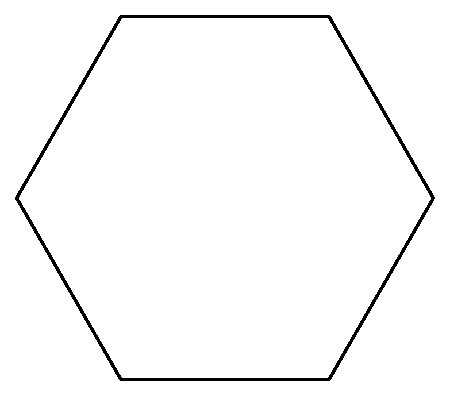
\includegraphics[width=2.5cm]{loopHexagon}}{A Regular Pentagon}\label{xp:loopH}
Draw a regular hexagon using the method \ct{timesRepeat:}. 
\end{exofigwithsize}


Once you have gotten the hang of it, try drawing a regular polygon with a very large number of sides. You may have to reduce the side length to make the figure fit on the screen. When 
the number of sides is large and the side length is small, the polygon will look like a circle. 


\section{Rediscovering the Pyramids}

Recall how you coded the outline of the pyramid of Saqqara in Experiment 3-5. You can simplify 
your code by using a loop, as shown in Script 7-5. 

\begin{exofigwithsize}[0.7]{\includegraphics[width=3.5cm]{loopPyramid}}{A Regular Pentagon}\label{xp:loopPyramid}
	| pica | 
	pica := Bot new. 
	5 timesRepeat: 
		[pica north. 
		pica go: 20. 
		pica east. 
		pica go: 20]. 
	5 timesRepeat: 
		[pica go: 20. 
		pica south. 
		pica go: 20. 
		pica east]. 
	pica west. 
	pica go: 200. 
\end{exofigwithsize}

Now you should be able to generate pyramids with an arbitrary number of terraces using 
the same number of expressions, merely by changing the numbers in the script. 

\begin{exofigwithsize}[0.7]{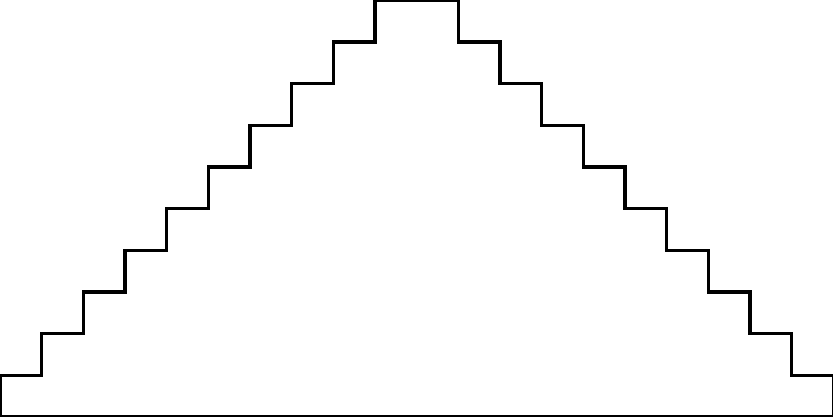
\includegraphics[width=3.5cm]{loopPyramid10}}{A Ten-Step Pyramid}\label{xp:loopPyramidten}
Draw a pyramid with 10 terraces using a variation of Script~\ref{scr:loopPyramid}. 
\end{exofigwithsize}

You may now want to generate pyramids with even larger numbers of terraces. The size of 
the terraces will have to be adjusted if you want them to fit on the screen. 

\section{Further Experiments with Loops}

As you have seen, generating a step pyramid involves the repetition of a block of code that 
draws two line segments. Once you have identified the proper repeating element, you can 
produce complex pictures from elementary drawings through repetition. The following 
experiments illustrate this principle. 



\ifx\wholebook\relax\else
    \end{document}
\fi


\section{Summary}
\noindent
{\small \begin{tabular}{p{20mm}p{50mm}p{30mm}}
\hline
\textbf{Method} & \textbf{Description} & \textbf{Example}\\
\hline
\textsf{lookLikeCircle} & Change the shape of the receiver to a circle. & \textsf{Bot new lookLikeCircle} \\

\textsf{lookLikeBot} & Change the shape of the receiver to a robot. & \textsf{Bot new lookLikeBot} \\

\textsf{lookLikeTriangle} & Change the shape of the receiver to a triangle. & \textsf{Bot new lookLikeTriangle} \\

\textsf{lookLikeImage} & Change the appearance of the receiver to the graphic you painted. & \textsf{Bot new lookLikeImage} \\

\textsf{lookLikeCircle} & Sending to the class results in newly created robots having the shape of a circle. 
& \textsf{Bot lookLikeCircle} \\

\textsf{lookLikeBot} & Sending to the class results in newly created robots having the shape of a robot. & \textsf{Bot lookLikeBot} \\

\textsf{lookLikeTriangle} & Sending to the class results in newly created robots having the shape of a triangle. 
& \textsf{Bot lookLikeTriangle} \\

\textsf{lookLikeImage} & Sending to the class results in newly created robots having the shape of the graphic you painted or loaded. & \textsf{Bot lookLikeImage} \\

\textsf{loadImage: '{\itshape fileName}'} & Load the image file \emph{fileName.frm} into the class or the robot.
& \textsf{Bot loadImage: 'spider'} \newline or \newline \textsf{berthe loadImage: 'spider'} \\

\textsf{loadImage} & Prompt the user for the name of an image file to be loaded into the class or the robot. 
& \textsf{Bot loadImage} or \newline  \textsf{berthe loadImage} \\

\textsf{saveImage: '{\itshape fileName}'} & Save the image of the class or the robot to the file named 
\emph{fileName.frm}. & \textsf{Bot saveImage: 'spider'} \newline or \newline  \textsf{berthe saveImage: 'spider'} \\

\textsf{saveImage} & Save the image of the class or the robot by prompting the user for a file name. 
& \textsf{Bot saveImage} or \newline  \textsf{berthe saveImage} \\

\textsf{penColor: {\itshape aColor}} & 
Change the color of the pen.
& \textsf{berthe penColor: Color blue} \\
\hline
\end{tabular}}

\noindent
{\small \begin{tabular}{p{20mm}p{50mm}p{30mm}}
\hline
\textbf{Method} & \textbf{Description} & \textbf{Example}\\
\hline

\textsf{penSize: {\itshape aNumber}} & 
Change the size of the pen. The default size is 1. 
& \textsf{berthe penSize: 3} \\

\textsf{color: {\itshape aColor}} & Change the color of the receiver to the specified color. 
& \textsf{berthe color: Color yellow} \\ 

\textsf{extent: {\itshape aPoint}} & Change the size of the receiver to dimensions given by \textsf{aPoint}
where \textsf{aPoint} is given by \textsf{w@h}, where \textsf{w} is the width and \textsf{h} is the height. & \textsf{berthe extent: 80@100} \\

 \textsf{passImageToClass} & Pass the graphic of the receiver to the class. After this message, robots created by the class will have as graphic the graphic of the current robot. & \textsf{berthe passImageToClass} \\
 
 \textsf{getImageFromClass} & Get the graphic of the class. After this message, the receiver will look like the robots that would be created by the class.  & \textsf{berthe getImageFromClass} \\
\hline
\end{tabular}}


%% %%%%%%%%%%%%%%%%%%%%%%%%%%%%%%%%%%%%%%%%%%%%%%%%%%%%%%%%%%%%%%%%%%%%%%%
% \begin{exofigwithsize}[0.5]{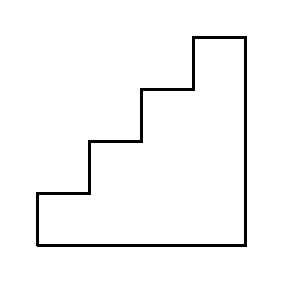
\includegraphics[width=3cm]{turtleMSmallStairs}}{A Staircase}\label{xp:letterA}
% You are not limited in your robot drawings to squares. You can create a wide range of geometrical figures.
% For example, here is a drawing of a small staircase. Write a script to reproduce this drawing. 
% \end{exofigwithsize}
% %%%%%%%%%%%%%%%%%%%%%%%%%%%%%%%%%%%%%%%%%%%%%%%%%%%%%%%%%%%%%%%%%%%%%%%%
% \begin{exonofigtitle}{Moving Clock Hands}
% Experiment with different angle values for each of the two robots; that is,change the angle values for the two turn 
% methods. Then, compare the effect of the method \ct{turnLeft: 60} (for pica) and \ct{turnRight: 300} (for daly). 
% You can see that turning left 60 degrees yields the same result as turning right 300 degrees. This is so because 
% the sum of the two values is 360 degrees, that is, a full circle. 
% \end{exonofigtitle}

\ifx\wholebook\relax\else
    \end{document}
\fi

%%% Local Variables:
%%% coding: utf-8
%%% mode: latex
%%% TeX-master: t
%%% TeX-PDF-mode: t
%%% ispell-local-dictionary: "english"
%%% End:
